\section{Durchführung und Auswertung}
Nachdem im letzten Versuchsteil die Kalibrierung der Energie über die Kanäle bestimmt wurde, werden nun sechs verschiedene, unbekannte Proben mithilfe der Rutherford-Backscattering-Methode auf ihre chemische Zusammensetzung analysiert. Aus den gemessenen Werten für die Rückstreuungsenergie kann so der K-Wert berechnet und mit den bekannten theoretischen K-Werten verglichen werden. Daraus lassen sich so die beinhalteten Elemente bestimmen. Die gemessenen Kanäle, Energien und K-Werte zusammen mit der Element-Bestimmung finden sich in den Tabellen \ref{Probe1} bis \ref{Probe6}. Die zugehörigen Spektren finden sich weiterhin in den Abbildungen \ref{Probe11} bis \ref{Münze1}. 

\begin{table}[h]
	\caption{Auswertung RBS - Probe 1}
	\begin{tabular}{|c|c|c|c|c|c|}
	\hline
	 & Mittl.Kanallage & Energie in keV & K-Faktor exp. & K-Faktor theo. & Element \\ \hline
	   1 & 692 & 1431 & 0,712 & 0,716 & Ti\\ \hline
	   2 & 529 & 1101 & 0,551 & 0,552 & Al \\ \hline
	\end{tabular}
\label{Probe1}
\end{table}

\begin{table}[h]
	\caption{Auswertung RBS - Probe 2}
	\begin{tabular}{|c|c|c|c|c|c|}
	\hline
	 & Mittl.Kanallage & Energie in keV & K-Faktor exp. & K-Faktor theo. & Element \\ \hline
	   1 & 818 & 1687 & 0,843 & 0,842 & Nb\\ \hline
	   2 & 693 & 1434 & 0,717 & 0,716 & Ti \\ \hline
	   3 & 526 & 1095 & 0,548 & 0,552 & Al \\ \hline
	\end{tabular}
\label{Probe2}
\end{table}

\begin{table}[h]
	\caption{Auswertung RBS - Probe 3}
	\begin{tabular}{|c|c|c|c|c|c|}
	\hline
	 & Mittl.Kanallage & Energie in keV & K-Faktor exp. & K-Faktor theo. & Element \\ \hline
	   1 & 532 & 1107 & 0,550 & 0,552 & Al\\ \hline
	   2 & 343 & 725 & 0,362 & 0,362 & O \\ \hline
	\end{tabular}
\label{Probe3}
\end{table}

\begin{table}[h]
	\caption{Auswertung RBS - Probe 4}
	\begin{tabular}{|c|c|c|c|c|c|}
	\hline
	 & Mittl.Kanallage & Energie in keV & K-Faktor exp. & K-Faktor theo. & Element \\ \hline
	   1 & 650 & 1346 & 0,673 & 0,674 & Ca\\ \hline
	   2 & 403 & 846 & 0,423 & 0,427 & F \\ \hline
	   3 & 237 & 510 & 0,255 & 0,252 & C \\ \hline
	\end{tabular}
\label{Probe4}
\end{table}

\begin{table}[h]
	\caption{Auswertung RBS - Probe 5 (Münze)}
	\begin{tabular}{|c|c|c|c|c|c|}
	\hline
	 & Mittl.Kanallage & Energie in keV & K-Faktor exp. & K-Faktor theo. & Element \\ \hline
	   1 & 745 & 1539 & 0,769 & 0,778 & Cu\\ \hline
	\end{tabular}
\label{Probe5}
\end{table}

\begin{table}[h]
	\caption{Auswertung RBS - Probe 1}
	\begin{tabular}{|c|c|c|c|c|c|}
	\hline
	 & Mittl.Kanallage & Energie in keV & K-Faktor exp. & K-Faktor theo. & Element \\ \hline
	   1 & 624 & 1294 & 0,647 & 0,637 & Cl\\ \hline
	   2 & 484 & 1010 & 0,505 & 0,497 & Na \\ \hline
	\end{tabular}
\label{Probe6}
\end{table}

Besonders auffällig stellt sich unsere Probe 5 dar, welche aus einer 1-Cent-Euro-Münze bestand. Laut \cite{muenze} bestehen die Centmünzen aus Stahl mit einer Kupferauflage. Die Kupferauflage können wir mit unserem Experiment sehr gut bestätigen, während der Hinweis auf den Stahlbestandteil der Münze ausbleibt. Wir vermuten, dass die vorhandene Kupferschicht wohl zu dick ist, sodass keine der Strahlen den Stahlkern erreichen. hier könnten wir die Energie des Strahls erhöhen, um eine höhere Eindringtiefe zu erreichen. Auch in Probe 4 ist weiterhin eine Besonderheit zu erkennen, da wir wieder eine geringer ausgeprägte Kante bei ca. 500keV sehen können. Wie schon im Abschnitt zur Kalibrierung besteht die Probe hierbei aus einer dünnen Element-Schicht auf einer Kohlenstoffbasis, welche hier erneut zum Vorschein kommt.


\begin{figure}[htbp] 
	\begin{minipage}[t]{0.45\linewidth} 
     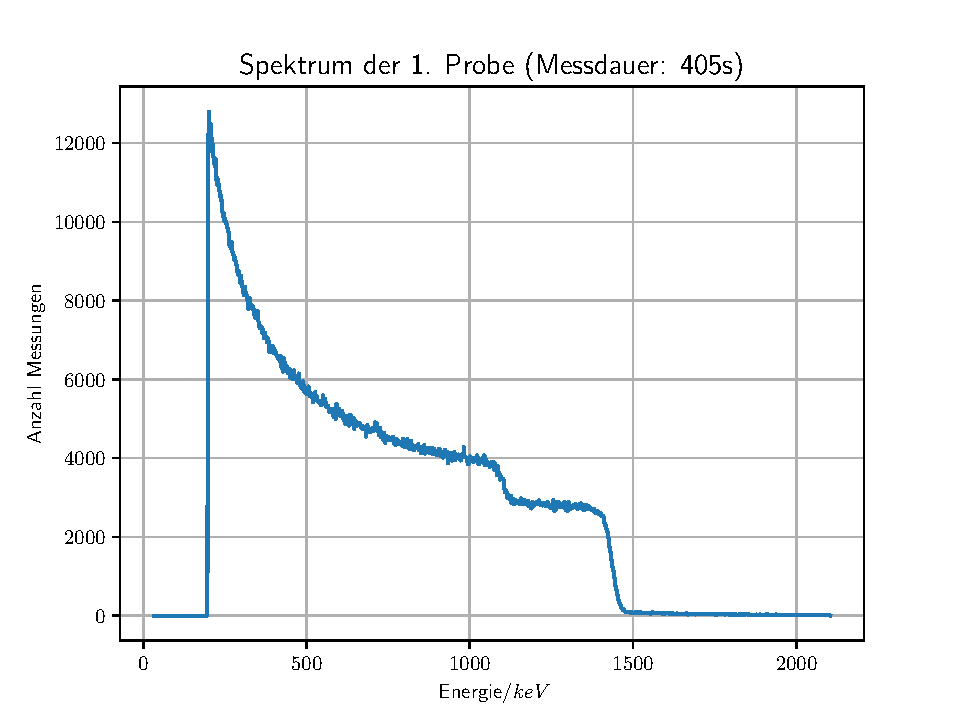
\includegraphics[scale=0.5]{1Probe.pdf}
  \caption{Spektrum 1. Probe}
  \label{Probe11}
\end{minipage}
\hfill
\begin{minipage}[t]{0.45\linewidth}  
     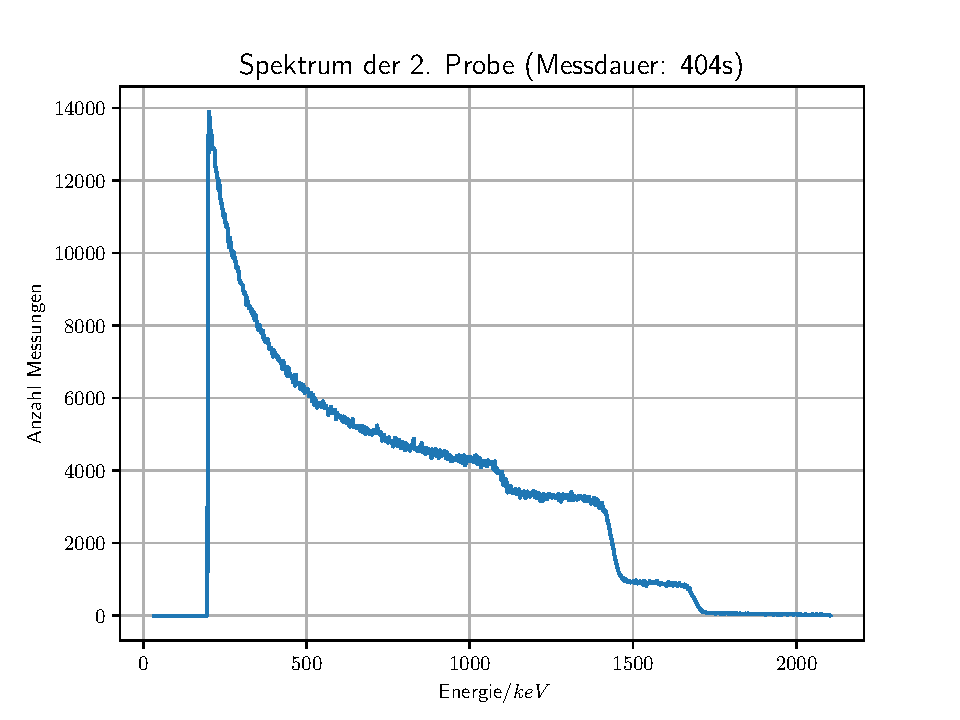
\includegraphics[scale=0.5]{2Probe.pdf}
  \caption{Spektrum 2. Probe}
  \label{Probe21}
\end{minipage}
\end{figure}

\begin{figure}[htbp] 
	\begin{minipage}[t]{0.45\linewidth} 
     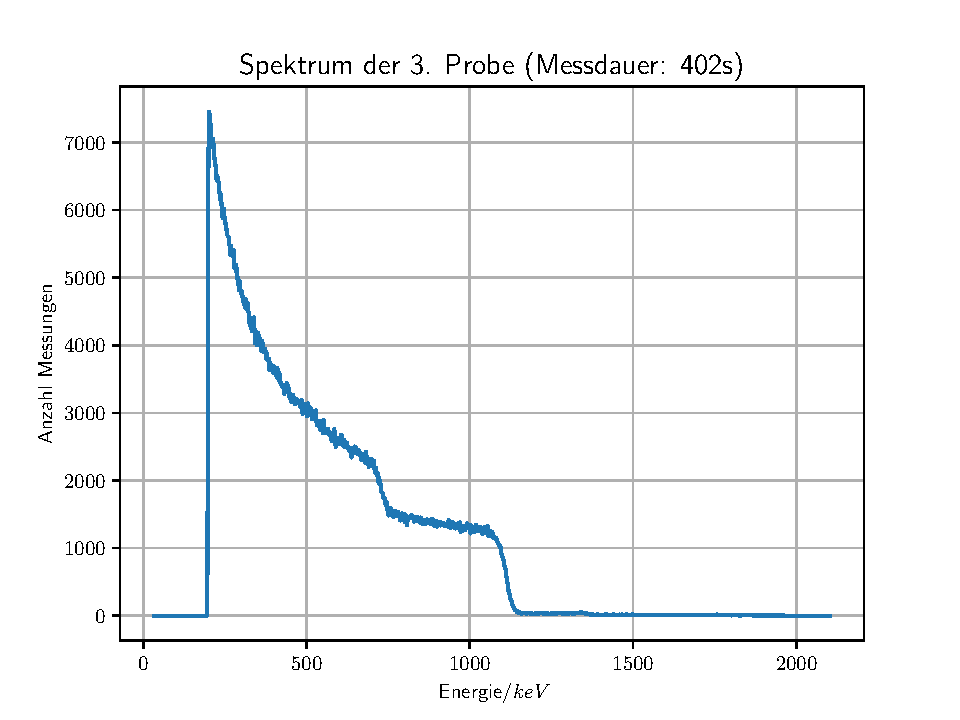
\includegraphics[scale=0.5]{3Probe.pdf}
  \caption{Spektrum 3. Probe}
  \label{Probe31}
\end{minipage}
\hfill
\begin{minipage}[t]{0.45\linewidth}  
     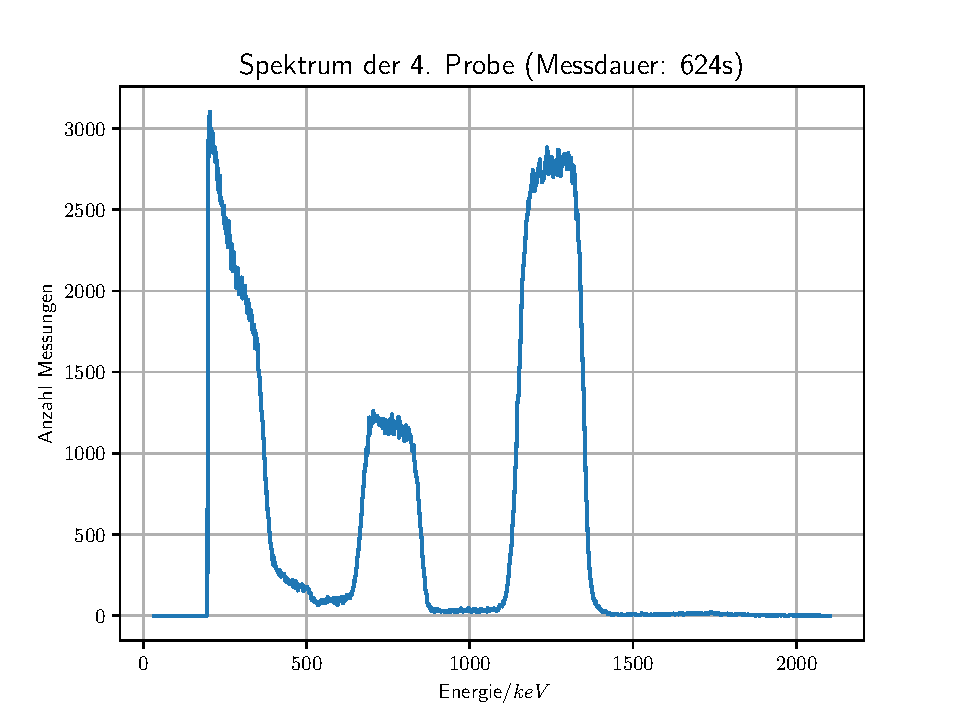
\includegraphics[scale=0.5]{4Probe.pdf}
  \caption{Spektrum 4. Probe}
  \label{Probe41}
\end{minipage}
\end{figure}

\begin{figure}[htbp] 
	\begin{minipage}[t]{0.45\linewidth} 
     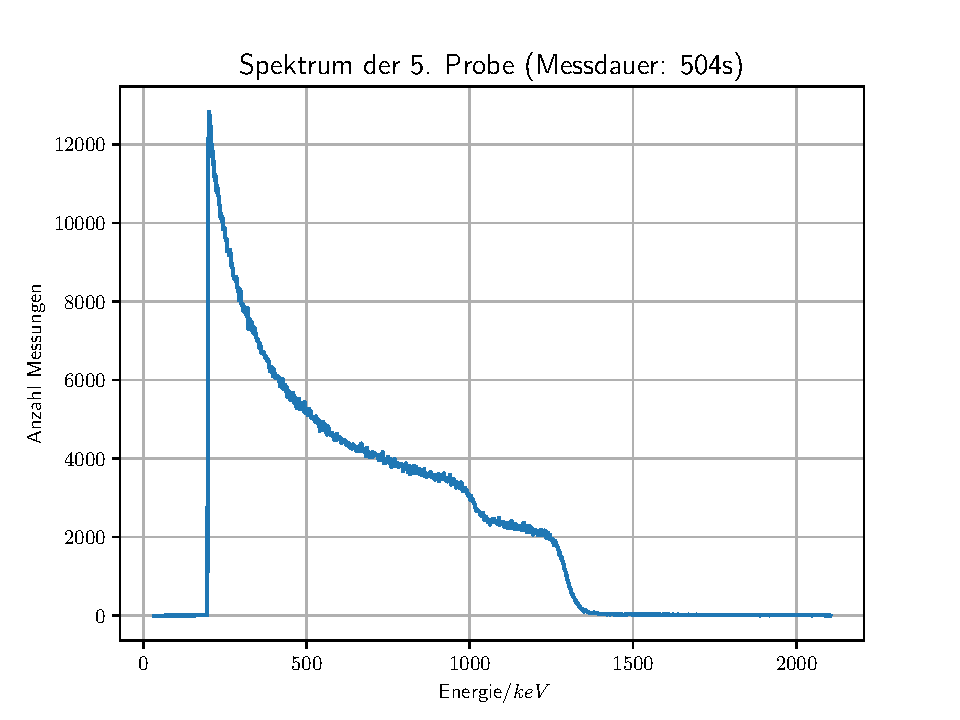
\includegraphics[scale=0.5]{5Probe.pdf}
  \caption{Spektrum 5. Probe}
  \label{Probe51}
\end{minipage}
\hfill
\begin{minipage}[t]{0.45\linewidth}  
     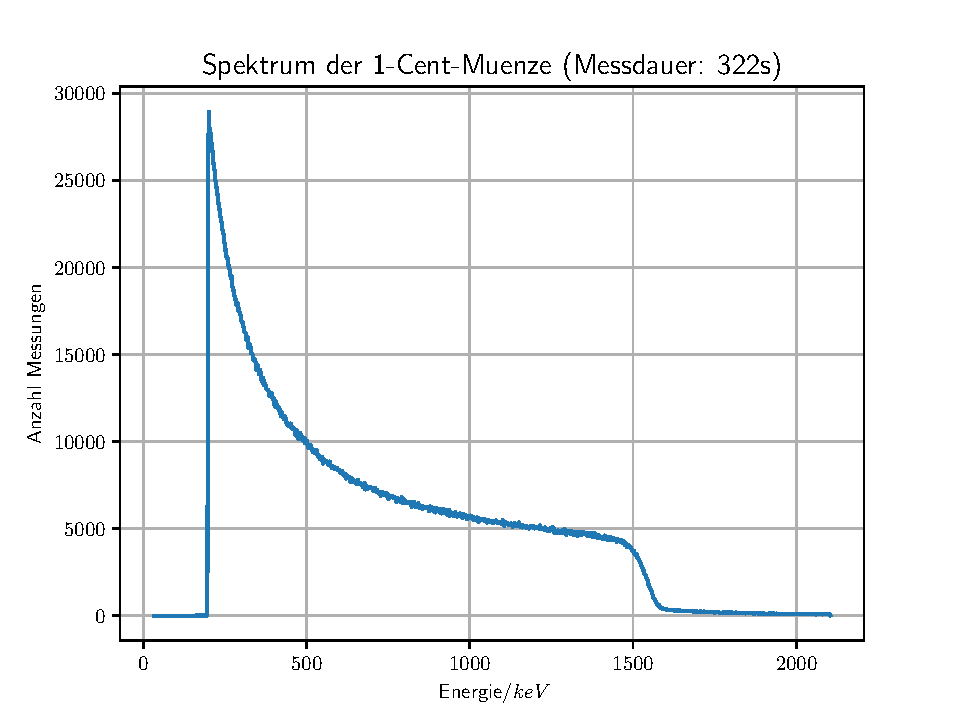
\includegraphics[scale=0.5]{1-Cent-Muenze.pdf}
  \caption{Spektrum 1-Cent-Münze}
  \label{Münze1}
\end{minipage}
\end{figure}
